\section{Metodologia}

Este capítulo aborda a metodologia de trabalho adotada para o desenvolvimento do projeto, desde a definição do tema até a conclusão dos objetivos propostos. Ela é baseada no modelo Cascata \cite{royce1987managing}, onde há uma correlação entre cada fase, e todo o processo é planejado antes de sua execução. A Figura \ref{fig:metodologia-simples} é uma representação gráfica da metodologia abordada.

\begin{figure}[H]
\centering
\caption{Metodologia abordada no projeto}
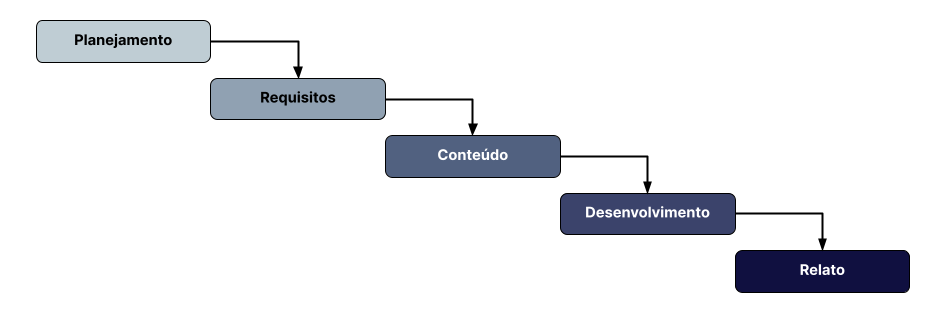
\includegraphics[width=1\textwidth]{figuras/imagens/metodologia-simples.png}
\legend {(Fonte: Elaborado pelo Autor)}
\label{fig:metodologia-simples}
\end{figure}

